% <--- percent sign starts a comment line in LaTeX

%----------------------------------------------------------
% This is a sample assignment .tex file. Put your name,
% assignment number and the due date below, as shown.
% Before you typeset your own assignment try to preview
% and print this one as follows:
%   1. Save this in a file, say hw.tex
%   2. do "latex hw"
%	3. latex will produce a pdf file that should be named hw.pdf.
%	4. Use any pdf viewer to view the document
% ------------------------------------------------------------

\documentclass[11pt]{article}

\usepackage{fullpage,graphicx,latexsym,picinpar,amsbsy,amsmath,amsfonts}

           

%%%%%%%%%%%%%%%%%%%%%%%%%%%%%%%%%%%%%%%%%%%%%%%%%%%%%%%%%%%%%%%%%%%%%%%%%%%%%%%%%%%
%%%%%%%%%%%  LETTERS 
%%%%%%%%%%%%%%%%%%%%%%%%%%%%%%%%%%%%%%%%%%%%%%%%%%%%%%%%%%%%%%%%%%%%%%%%%%%%%%%%%%%

\newcommand{\barx}{{\bar x}}
\newcommand{\bary}{{\bar y}}
\newcommand{\barz}{{\bar z}}
\newcommand{\bart}{{\bar t}}

\newcommand{\bfP}{{\bf{P}}}

%%%%%%%%%%%%%%%%%%%%%%%%%%%%%%%%%%%%%%%%%%%%%%%%%%%%%%%%%%%%%%%%%%%%%%%%%%%%%%%%%%%
%%%%%%%%%%%%%%%%%%%%%%%%%%%%%%%%%%%%%%%%%%%%%%%%%%%%%%%%%%%%%%%%%%%%%%%%%%%%%%%%%%%
                                                                                
\newcommand{\parend}[1]{{\left( #1  \right) }}
\newcommand{\spparend}[1]{{\left(\, #1  \,\right) }}
\newcommand{\angled}[1]{{\left\langle #1  \right\rangle }}
\newcommand{\brackd}[1]{{\left[ #1  \right] }}
\newcommand{\spbrackd}[1]{{\left[\, #1  \,\right] }}
\newcommand{\braced}[1]{{\left\{ #1  \right\} }}
\newcommand{\leftbraced}[1]{{\left\{ #1  \right. }}
\newcommand{\floor}[1]{{\left\lfloor #1\right\rfloor}}
\newcommand{\ceiling}[1]{{\left\lceil #1\right\rceil}}
\newcommand{\barred}[1]{{\left|#1\right|}}
\newcommand{\doublebarred}[1]{{\left|\left|#1\right|\right|}}
\newcommand{\spaced}[1]{{\, #1\, }}
\newcommand{\suchthat}{{\spaced{|}}}
\newcommand{\numof}{{\sharp}}
\newcommand{\assign}{{\,\leftarrow\,}}
\newcommand{\myaccept}{{\mbox{\tiny accept}}}
\newcommand{\myreject}{{\mbox{\tiny reject}}}
\newcommand{\blanksymbol}{{\sqcup}}
                                                                                                                         
\newcommand{\veps}{{\varepsilon}}
\newcommand{\Sigmastar}{{\Sigma^\ast}}
                           
\newcommand{\half}{\mbox{$\frac{1}{2}$}}    
\newcommand{\threehalfs}{\mbox{$\frac{3}{2}$}}   
\newcommand{\domino}[2]{\left[\frac{#1}{#2}\right]}  

%%%%%%%%%%%% complexity classes

\newcommand{\PP}{\mathbb{P}}
\newcommand{\NP}{\mathbb{NP}}
\newcommand{\PSPACE}{\mathbb{PSPACE}}
\newcommand{\coNP}{\textrm{co}\mathbb{NP}}
\newcommand{\DLOG}{\mathbb{L}}
\newcommand{\NLOG}{\mathbb{NL}}
\newcommand{\NL}{\mathbb{NL}}

%%%%%%%%%%% decision problems

\newcommand{\PCP}{\sc{PCP}}
\newcommand{\Path}{\sc{Path}}
\newcommand{\GenGeo}{\sc{Generalized Geography}}

\newcommand{\malytm}{{\mbox{\tiny TM}}}
\newcommand{\malycfg}{{\mbox{\tiny CFG}}}
\newcommand{\Atm}{\mbox{\rm A}_\malytm}
\newcommand{\complAtm}{{\overline{\mbox{\rm A}}}_\malytm}
\newcommand{\AllCFG}{{\mbox{\sc All}}_\malycfg}
\newcommand{\complAllCFG}{{\overline{\mbox{\sc All}}}_\malycfg}
\newcommand{\complL}{{\bar L}}
\newcommand{\TQBF}{\mbox{\sc TQBF}}
\newcommand{\SAT}{\mbox{\sc SAT}}

%%%%%%%%%%%%%%%%%%%%%%%%%%%%%%%%%%%%%%%%%%%%%%%%%%%%%%%%%%%%%%%%%%%%%%%%%%%%%%%%%%%
%%%%%%%%%%%%%%% for homeworks
%%%%%%%%%%%%%%%%%%%%%%%%%%%%%%%%%%%%%%%%%%%%%%%%%%%%%%%%%%%%%%%%%%%%%%%%%%%%%%%%%%%

\newcommand{\student}[2]{%
{\noindent\Large{ \emph{#1} SID {#2} } \hfill} \vskip 0.1in}

\newcommand{\assignment}[1]{\medskip\centerline{\large\bf CS 111 ASSIGNMENT {#1}}}

\newcommand{\duedate}[1]{{\centerline{due {#1}\medskip}}}     

\newcounter{problemnumber}                                                                                 

\newenvironment{problem}{{\vskip 0.1in \noindent
              \bf Problem~\addtocounter{problemnumber}{1}\arabic{problemnumber}:}}{}

\newcounter{solutionnumber}

\newenvironment{solution}{{\vskip 0.1in \noindent
             \bf Solution~\addtocounter{solutionnumber}{1}\arabic{solutionnumber}:}}
				{\ \newline\smallskip\lineacross\smallskip}

\newcommand{\lineacross}{\noindent\mbox{}\hrulefill\mbox{}}

\newcommand{\decproblem}[3]{%
\medskip
\noindent
\begin{list}{\hfill}{\setlength{\labelsep}{0in}
                       \setlength{\topsep}{0in}
                       \setlength{\partopsep}{0in}
                       \setlength{\leftmargin}{0in}
                       \setlength{\listparindent}{0in}
                       \setlength{\labelwidth}{0.5in}
                       \setlength{\itemindent}{0in}
                       \setlength{\itemsep}{0in}
                     }
\item{{{\sc{#1}}:}}
                \begin{list}{\hfill}{\setlength{\labelsep}{0.1in}
                       \setlength{\topsep}{0in}
                       \setlength{\partopsep}{0in}
                       \setlength{\leftmargin}{0.5in}
                       \setlength{\labelwidth}{0.5in}
                       \setlength{\listparindent}{0in}
                       \setlength{\itemindent}{0in}
                       \setlength{\itemsep}{0in}
                       }
                \item{{\em Instance:\ }}{#2}
                \item{{\em Query:\ }}{#3}
                \end{list}
\end{list}
\medskip
}

%%%%%%%%%%%%%%%%%%%%%%%%%%%%%%%%%%%%%%%%%%%%%%%%%%%%%%%%%%%%%%%%%%%%%%%%%%%%%%%%%%%
%%%%%%%%%%%%% for quizzes
%%%%%%%%%%%%%%%%%%%%%%%%%%%%%%%%%%%%%%%%%%%%%%%%%%%%%%%%%%%%%%%%%%%%%%%%%%%%%%%%%%%

\newcommand{\quizheader}{ {\large NAME: \hskip 3in SID:\hfill}
                                \newline\lineacross \medskip }


%%%%%%%%%%%%%%%%%%%%%%%%%%%%%%%%%%%%%%%%%%%%%%%%%%%%%%%%%%%%%%%%%%%%%%%%%%%%%%%%%%%
%%%%%%%%%%%%% for final
%%%%%%%%%%%%%%%%%%%%%%%%%%%%%%%%%%%%%%%%%%%%%%%%%%%%%%%%%%%%%%%%%%%%%%%%%%%%%%%%%%%

\newcommand{\namespace}{\noindent{\Large NAME: \hfill SID:\hskip 1.5in\ }\\\medskip\noindent\mbox{}\hrulefill\mbox{}}



\begin{document}

% v -- YOUR NAME and SID in the braces
\student{ Chris Wong}{ 860 923 521 }
% v -- ASSIGNMENT NUMBER in the braces
\assignment{ 3 }
% v-- DUE DATE in the braces
\duedate{5/10/2011 }

\medskip

%%%%%%%%%%%%%%%%%%%%%%%%%%%%%%%%%%%%%%%%%%%%%%%%%%%%%%%%%%%%%%%%%%%%%%%%%%

\lineacross

%%%%%%%%%%%%%%%%%%%%%%%%%%%%

\begin{problem}
	We construct recursively binary trees $T_0, T_1, T_2, ...$,
as follows. Both $T_0$ and $T_1$ consist of a single node.
For $n\ge 2$, to obtain $T_n$, we link
one copy of $T_{n-1}$ and two copies of
$T_{n-2}$, as in the figure below:

\begin{center}
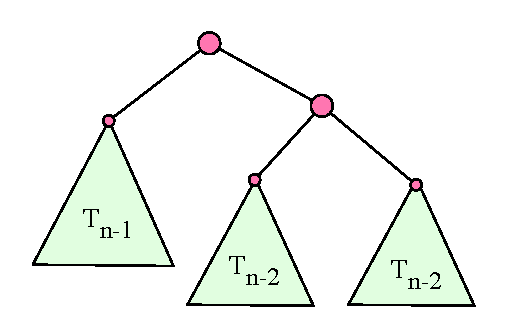
\includegraphics[width=2.5in]{hw3_bin_tree.pdf}
\end{center}

Let $b_n$ be the number of nodes in $T_n$. For example,
$b_0 = 1$, $b_1 = 1$, $b_2 = 5$ and $b_3 = 9$. Give the
formula for $b_n$. Show your work.  The solution
must consist of the following steps:
(i) Set up a recurrence equation and give a brief justification.
(ii) Give the associated homogeneous equation.
(iii) Determine the characteristic equation and solve it.
(iv) Give the general solution for the homogeneous equation.
(v) Determine a particular solution for the non-homogeneous equation.
(vi) Give the general solution for the non-homogeneous equation.
(vii) Use the initial conditions to compute the final answer.
\end{problem}

%---------------------------

\pagebreak
\begin{solution}
	\\i) First, lets count the number nodes and recurances in the tree. There are
	two nodes, one $T_{n-1}$ recurrance, and two $T_{n-2}$ recurannces. Now can
	derive the recurrance eqaution: \\$b(n) = T_{n-1} + 2T_{n-2} + 2$
	\\
	\\ii)Homogeneous equation: $Tn = T_{n-1} + 2T_{n-2}$
	\\
	\\iii)Characteristic equation: $x^{2} - x - 2 = 0$ then $(x-2)(x+1)$
	So, roots = 2 and -1
	\\
	\\iv)General soultion: b(n) = $C_{1}(2)^{n} + C_{2}(-1)^{n} + Y_{p}$(particular sol.)
	\\
	\\v)Non-homogeneous equation:$Tn = T_{n-1} + 2T_{n-2} + 2$ $\Rightarrow$
	$A=A+ 2A + 2 $ $\Rightarrow$ $A = -1$ So, particular solution = -1
	\\
	\\vi)General solution = Characteristic solution + Particular solution $\Rightarrow$
	$C_{1}(2)^{n} + C_{2}(-1)^{n} - 1$
	\\
	\\vii)Plugging in:
	\\$b_0 = 1$ $\Rightarrow$ $1 = C_{1} + C_{2} - 1 $
	\\$b_1 = 1$ $\Rightarrow$ $1 = (2)C_{1} + (-1)C_{2} - 1 $
	\\$C_{1} = \frac{4}{3} , C_{2} = \frac{2}{3}$
	\\Thus, the final answer is: $b(n) = \frac{4}{3}(2)^{n} + \frac{2}{3}(-1)^{n} - 1$
\end{solution}

%%%%%%%%%%%%%%%%%%%%%%%%%%%%
\pagebreak
\begin{problem}
	Let $S_n$ be the number of tilings of the $n\times 3$ grid with
$1\times 3$ and $2\times 3$ tiles. (Tiles can be rotated by 90 degrees.)
 Give a recurrence relation
for $S_n$ and justify its correctness.

Note: This recurrence will be of degree higher than $2$, and you
\emph{do not} have to solve it. The reverse page shows all tilings of
the $5\times 3$ grid, showing that $S_5 = 23$. You can use this value to
verify you recurrence.
\end{problem}

%-----------------------------

\begin{solution}
\\   First,  set n = 1. So, we will find the number of times a 1x3 and 2x3 fits
into a 1x3 square. Only one 1x3 piece can fit into a 1x3. no 2x3 pieces can fit
inside a 1x3. Those there exists only one possible combination for n=1
\\
\\   Next set n = 2. So, we will find the number of times a 1x3 and 2x3 fits
into a 2x3 square without repitions from previous answers.  Two 1x3 pieces can fit
insde a 2x3, but this is a repition of n=1, so we will not count that combination.
A single 2x3 piece will fit inside a 2x3, and those are the only possible combinations.
Thus, there exists only one more combination for n=2
\\
\\   Third, we set n = 3. So we will find the number of times a 1x3 and 2x3 fits
into a 3x3 square without repitions from pervious n's. Three horizontal 1x3's,
one 1x3 followed by a 2x3 horizontal, and a 2x3 followed by a 1x3 horizontal are
the possible combinations that exist.  There are more, but those are just repeats
of the pervious n's. So, there exsits 3 combinations for n = 3
\\
\\   There are no new combinations for n > 3 because of repition. We can now
derive the recurrence relation: $S_{n} = S_{n-1} + S_{n-2} + 3S_{n-3}$
\end{solution}

%%%%%%%%%%%%%%%%%%%%%%%%%%%

\begin{problem}
    No partner
\end{problem}

%----------------------------

\begin{solution}
    No partner
\end{solution}

\end{document}
